\chapter{Network Layer - Piano di controllo}

\section{Algoritmi di Instradamento (routing)}
Lo scopo di questi algoritmi è \textbf{determinare i migliori cammini} da usare dalle sorgenti ai destinatari. Il miglior cammino è valutato rispetto a vari fattori, che riprendono ciò che abbiamo affrontato nello studio dei problemi di ottimizzazione sui grafi, nella materia Algoritmi e Laboratorio. \href{https://github.com/BoredDam/Algoritmi}{Vedi il mio GitHub per approfondimenti}.

\begin{itemize}
	\item \textit{Shortest path}, o \textit{shortest unweighted path}.\\
	Il cammino, da nodo $A$ a nodo $B$ che passa attraverso il \textbf{minor numero di nodi}.
	
	\item \textit{Shortest weighted path}, o \textit{least-cost path}.\\
	Il cammino $p= \langle (v_1, v_2), (v_2, v_3) \dots, (v_{n-1},v_n) \rangle$ tale che $A=v_1$, $B = v_n$ e 
	$$
	\min \sum_{i=1}^n c(v_{i-1}, v_i)
	$$
	ovvero, tale che la \textbf{somma dei pesi} (o costi) del cammino da $A$ a $B$ sia \textbf{minima}.
\end{itemize}

Nonostante ciò, esistono molti altri fattori da \textbf{tenere in considerazione}, come \textbf{policy} di inoltro.

\subsection{Centralizzati, non centralizzati}
\begin{itemize}
	\item Un \textbf{algoritmo di instradamento centralizzato}, calcola il percorso migliore avendo una\\ conoscenza globale della rete. Ciò implica l'esistenza di un modo per conoscere i costi e la topologia relativi ad una rete. Il calcolo dei percorsi potrà poi essere effettuato da una struttura centralizzata e condiviso ai router, o replicato in ogni router.\\
	Un esempio di algoritmo a informazioni globali (centralizzato), è \textbf{l'algoritmo link-state}.
	
	\item Un \textbf{algoritmo di instradamento decentralizzato}, effettua lo stesso calcolo in maniera distribuita e iterativa. Nessun nodo possiede informazioni di tipo globale relative alla rete, ma solo quelle relative ai collegamenti adiacenti. Lo scambio di informazioni permette gradualmente di valutare il percorso a distanza minima. L'algoritmo decentralizzato che tratteremo sfrutta un vettore, chiamato \textbf{vettore delle distanze}, presente in ogni router, e che contiene al suo interno le stime relative alla lunghezza dei cammini minimi. È detto algoritmo \textbf{distance-vector}.
\end{itemize}

\subsection{Algoritmi statici e dinamici}
\begin{itemize}
	\item Negli \textbf{algoritmi di instradamento statici}, raramente i percorsi stabiliti cambiano. Solitamente ciò avviene sotto intervento umano.
	\item Negli \textbf{algoritmi di instradamento dinamici}, gli instradamenti variano in funzione di fattori quali volume del traffico, topologia della rete. L'algoritmo viene eseguito periodicamente o in funzione di variazioni nella topologia o di costi relativi ai collegamenti.
\end{itemize}
\newpage

\subsection{Algoritmi sensibili o insensibili al carico}
\begin{itemize}
	\item Gli \textbf{algoritmi sensibili al carico} usano il tasso di congestione dei collegamenti come criterio per valutarne il costo. Rispondono meglio ai cambiamenti della rete, ma sono molto sensibili a instradamento in loop e oscillazione dei percorsi.
	
	\item Gli \textbf{algoritmi insensibili al carico} non valutano gli stessi fattori.
\end{itemize}


Un'intuizione iniziale potrebbe farci preferire i primi ai secondi. Tuttavia, il costo di un collegamento calcolato in un momento di congestione, non esprime quello che dovrebbe essere il suo costo in condizioni normali. La congestione di rete potrebbe non durare abbastanza per rendere valida la scelta di un cammino migliore in quell'istante di tempo. Per Internet, si è preferito sfruttare algoritmi di instradamento insensibili al carico.

\subsubsection{Problema delle oscillazioni}
Negli algoritmi sensibili al carico appena accennati, si rischia lo scenario delle \textbf{oscillazioni dei percorsi}. Avviene quando il costo del collegamento è \textbf{pari al traffico trasportato}.

\begin{figure}[htp]
	\centering
	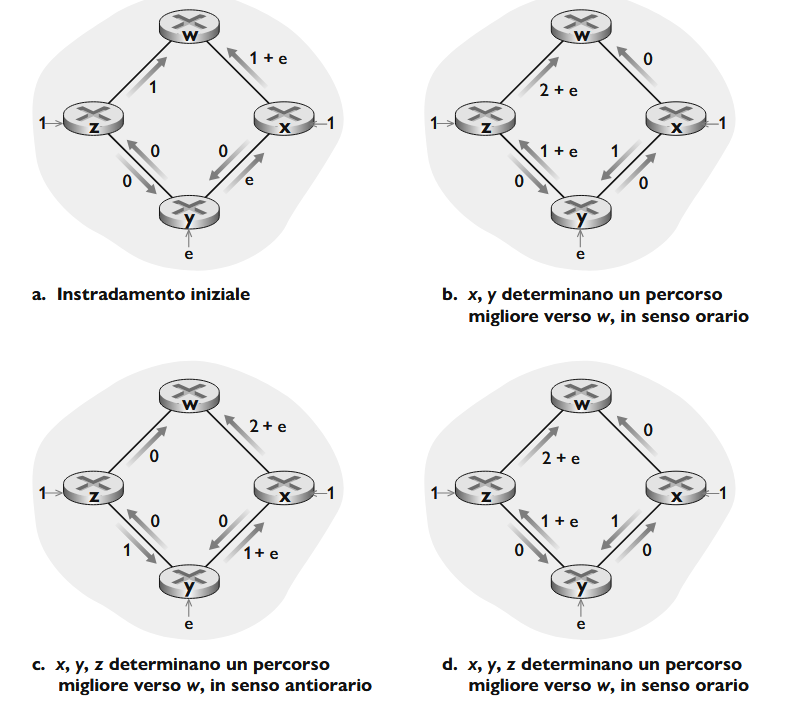
\includegraphics[width=0.75\linewidth]{./images/oscillazione dei percorsi.png}
\end{figure}

Questo scenario, causa cicli di ricalcolo continui che compromettono la stabilità dell'instradamento. La soluzione generale, consiste nell'\textbf{evitare che tutti i router eseguano l'algoritmo di routing allo stesso istante}.
\newpage

\section{Instradamento link-state}
Un \textbf{algoritmo di instradamento centralizzato}, calcola il percorso migliore avendo una conoscenza globale della rete.

\subsection{Flooding e Link state broadcast}
Conoscere la topologia e i costi della rete è quindi fondamentale per effettuare tutti i calcoli necessari. Il protocollo \textbf{Open Shortest Path First} (OSPF), sfrutta il \textbf{link-state broadcast}, ovvero l'invio di un particolare tipo di messaggio, chiamato \textbf{link-state advertisement} che viene distribuito nella rete tramite una tecnica chiamata \textbf{flooding}.

\subsubsection{Flooding}
È un protocollo di instradamento usato dai router: questi \textbf{inoltrano un pacchetto} in ingresso \textbf{su tutte le linee ad eccezione di quella da cui proviene}. Viene usato per \textbf{studiare la topologia della rete} e condividere tra i nodi informazioni relative ai \textbf{costi}.

\begin{figure}[htp]
	\centering
	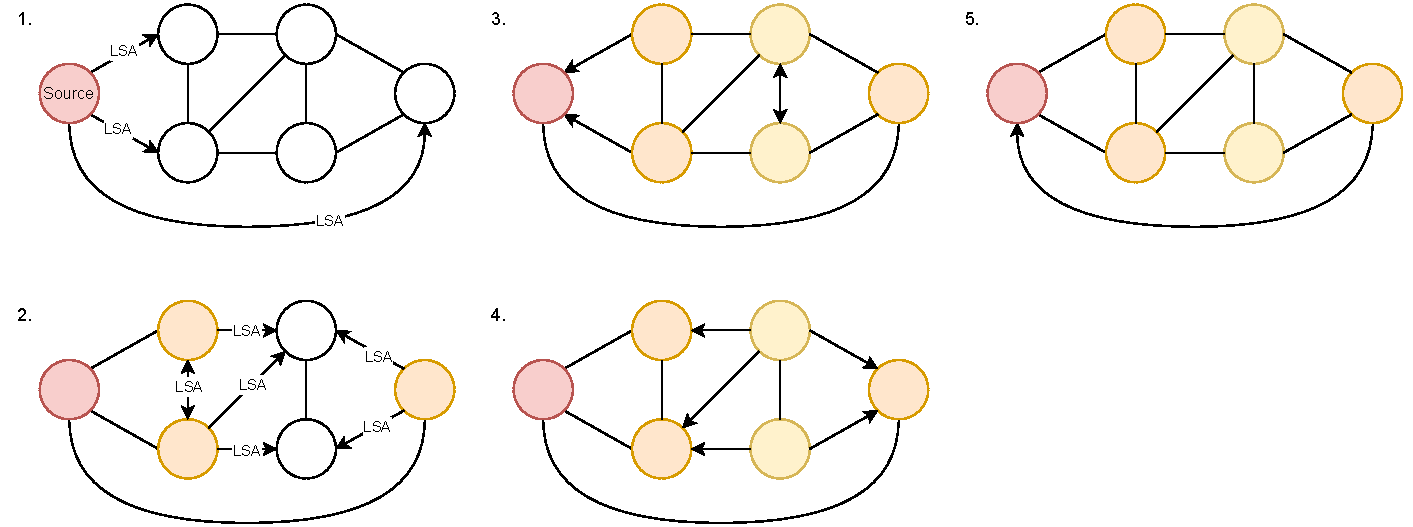
\includegraphics[width=1\linewidth]{./images/flooding.drawio.pdf}
\end{figure}

In reti più complesse e con più cicli, il flooding può creare un numero enorme di pacchetti duplicati, che potrebbero saturare la rete. È quindi consigliato introdurre dei meccanismi che controllino il flooding, come i seguenti:
\begin{itemize}
	\item ID per pacchetto, per evitare i duplicati.
	\item Impostare un limite di hop.
	\item Rimuovere i cicli dal grafo della rete.
	\item Inoltrare i messaggi solo lungo uno spanning tree.
\end{itemize}

\newpage

\subsection{Alcune convenzioni}
\begin{itemize}
	\item $G$ è il grafo.
	
	\item $G.V$ è l'insieme dei nodi del grafo, $G.E$ l'insieme degli archi. $w$ è una funzione (o una struttura dati contenente il) peso, che stabilisce il costo di un arco che unisce due nodi adiacenti.
	
	\item $d.v$ indica il costo minimo stimata dal nodo sorgente nell'iterazione corrente. Parte sempre da $+\infty$, tranne per il nodo sorgente, per cui $d.s = 0$.
	
	\item $\delta(s,v)$ indica l'effettivo costo del cammino minimo dal nodo sorgente a $v$. Presumibilmente, il nostro obiettivo sarà ottenere $d.v = \delta (s,v) \ \forall v \in G.V$.
	
	\item $p.v$ è il predecessore di $v$ all'interno del cammino di costo minimo dal nodo sorgente $s$.
	
	
\end{itemize}
\subsection{L'algoritmo di Dijkstra}
Dato in input un grafo $G$, un nodo sorgente $s$ e una struttura dati contenenti gli archi e il loro peso $w$, Dijkstra calcola tutti i cammini minimi che partono da $s$, verso ogni nodo $v \in G.V$.\\
Si suddivide in due fasi.

\subsubsection{Inizializzazione}
\begin{enumerate}
	
	\item Si pone $d.v= +\infty$ su tutti i nodi, tranne per il nodo sorgente $s$, per cui $d.s=0$.
	
	\item Si pone come $p.v = null$ per ogni nodo.
	
	\item Si crea un insieme $S = \varnothing$, che conterrà tutti i nodi di cui si conosce il cammino di peso minimo da $s$, inizialmente vuoto. Lo utilizzeremo nel corso dell'algoritmo.
	
	\item Si crea una struttura dati $Q = \varnothing$, di cui parleremo meglio dopo.
	
	\item Si inseriscono tutti i nodi all'interno di $Q$.
\end{enumerate}

\subsubsection{Iterazione}
\begin{enumerate}
	\item A ogni passaggio, estrarre il nodo $u$ con $d.u$ minimo da $Q$.\\
	Alla prima iterazione, il nodo estratto sarà $s$.
	
	\item Inserisci $u$ nell'insieme $S$.
	
	\item Verifica se è possibile ridurre $d.v$ dei nodi $v$ adiacenti ad $u$, passando proprio dal nodo $u$. La verifica si ripete su ogni nodo adiacente ad $u$. 
	
	\item Se l'insieme $S = G.V$, smetti di iterare, altrimenti torna al passo 1 dell'iterazione.
\end{enumerate}
Nota bene: ogni volta che è possibile ridurre $d.v$ passando da $u$, bisogna aggiornare il contenuto di $Q$.


\subsection{Complessità dell'algoritmo}
$Q$ sarà una struttura dati su cui effettuare operazioni di inserimento (all'inizio dell'algoritmo), estrazione del minimo e aggiornamento delle chiavi. Definiamo $Q$ come una \textbf{coda con priorità}. L'implementazione di $Q$ influenzerà la complessità dell'algoritmo.
\begin{itemize}
	\item Con $Q$ implementato con un array semplice, avremo una complessità $O(|V|^2)$.
	\item Con $Q$ implementato con un min-heap, si otterrà una complessità $O(|V|+|E|\log|V|)$.
\end{itemize}



\newpage

\section{Instradamento Distance Vector}
L'algoritmo distance-vector sfrutta l'algoritmo \textbf{Bellman-Ford}, creando un nuovo algoritmo asincrono, che girerà sui singoli nodi della rete. Proprio per questo motivo, introduciamo una notazione $D_x[v]$. $D_x$ è il vettore delle distanze, e $D_x[v]$ è la distanza stimata da $x$ a $v$.

\subsection{Algoritmo}
Su ciascun nodo $x \in G.V$ , girerà il seguente algoritmo:
\subsubsection{Inizializzazione}
\begin{enumerate}
	\item $D_x[x]=0$. Il nodo $x$ dista 0 da se stesso. 
	
	\item $\forall v \in G, \ D_x[y] =w (x,y)$. Chiaramente, se $u$ non è adiacente ad $x$, $D_x[u]= +\infty$
	
	\item Inoltra $D_x$ a tutti i nodi adiacenti.
\end{enumerate}

\subsubsection{Iterazione}
\begin{enumerate}
	\item Aspetta fino a quando non ricevi un vettore delle distanze, o finché non cambia il costo verso un nodo adiacente.
	
	\item Ricevuto il vettore delle distanze da un nodo $D_y$, si andrà a calcolare, per ogni $v \in G.V$, 
	$$
	D_x[v] = \min \{D_x[v], \;D_y[v] + w(x,y)\}
	$$
	ovvero, se esiste, calcolo il cammino di peso inferiore per andare da $x$ a $v$, passando per $y$. Se questa condizione si verifica, e la $D_x[v]$ di qualsiasi nodo $v$ cambia, inoltra al vettore delle distanze a tutti i nodi adiacenti.
	
	\item Ritorna allo step 1 dell'iterazione.
\end{enumerate}
Questo algoritmo è un algoritmo \textbf{asincrono}, che\textbf{ itera un numero indefinito di volte su ogni nodo}, in cui i valori minimi calcolati non cambiano, se non successivamente a cambiamenti della rete. In tal caso, ogni nodo cui vettore delle distanze cambia, inoltrerà quest'ultimo agli adiacenti.

\subsection{Poisoned reverse}
Esistono però delle \textbf{circostanze problematiche}, causate dalla \textbf{visibilità limitata} di ogni nodo rispetto ai costi complessivi \textbf{della rete}, che potrebbero causare \textbf{loop di inoltro di pacchetto}. In tal caso, si può introdurre un meccanismo di \textbf{poisoned reverse}, che permette ad un nodo $x$ di mentire a $y$ in una circostanza del genere:
\begin{enumerate}
	\item $y$: voglio inoltrare un pacchetto a $z$ per arrivare a $x$, perché costa meno.
	\item $z$: voglio inoltrare un pacchetto a $y$ per arrivare a $x$, perché costa meno.
\end{enumerate}
Si può arrivare a questa circostanza quando il peso di un arco non adiacente a $z$, ma adiacente a $y$, varia. In tal caso, $z$ vedrà che $y$ vuole arrivare ad $x$ passando da se stesso, osserva che lui farebbe l'opposto, e allora "mente" a $y$ dandogli un costo fittizio $D_z[x]=+\infty$, interrompendo il loop.

\newpage

\section{Routing in Internet}
Per facilitare il routing in Internet, quest'ultimo è organizzato in \textbf{sistemi autonomi} (AS). Ogni sistema autonomo è trattato come una singola entità amministrativa. 
\begin{itemize}
	\item All'interno di sistema autonomo, tutti i router eseguono lo stesso algoritmo di routing, chiamato \textbf{protocollo di instradamento intra-AS}.
	\item Per l‘instradamento tra AS distinti si usano invece \textbf{protocolli di instradamento inter-AS}.
\end{itemize} 
Questa organizzazione in sistemi autonomi, garantisce una maggiore \textbf{autonomia amministrativa} e migliore \textbf{scalabilità}. Ogni sistema autonomo è identificato da un \textbf{numero di sistema autonomo (ASN)}.

\subsection{RIP - Routing Information Protocol (intra-AS)}
È un protocollo di routing basato sull'algoritmo \textbf{Distance Vector} (Bellman-Ford) per il routing interno ai sistemi autonomi. La sua metrica è il \textbf{numero di hop}, ovvero il numero di router da attraversare per raggiungere una determinata destinazione.
\begin{itemize}
	\item Supporta al più 15 hop. Una destinazione $x$ con $d.x=16 \ \text{hop}$ è irraggiungibile.
	\item I router scambiano informazioni relative alle tabelle di routing ogni 30 secondi.
	\item Un percorso non aggiornato per 180 secondi è marcato come irraggiugibile.
	\item Dopo altri 120 secondi viene rimosso dalla tabella (garbage collection).
\end{itemize}
Sfrutta inoltre due tipi di messaggi:
\begin{itemize}
	\item \verb|REQUEST| per richiedere informazioni di routing ai router vicini.
	\item \verb|RESPONSE| per fornire aggiornamenti sulla propria tabella di routing.
\end{itemize}
\subsubsection{Tabelle di routing RIP}
Contengono:
\begin{itemize}
	\item Indirizzo $x$ di destinazione.
	\item Distanza minima (in hop) verso $x$.
	\item Prossimo hop per arrivare a $x$.
	\item Un timeout.
	\item Un timer per la garbage collection.
\end{itemize}

\subsubsection{Versioni di RIP}
\begin{itemize}
	\item \textbf{RIP v1} supporta solo indirizzamento classful senza subnet. Il campo next hop non è esplicito, e non supporta autenticazione.
	\item \textbf{RIP v2} supporta CIDR, Poison Reverse, autenticazione e next hop esplicito nel messaggio.
	\item \textbf{RIPng} (next generation) per IPv6, basata su RIP v2. Non supporta l'autenticazione.
\end{itemize}

\newpage

\subsection{OSPF - Open Shortest Path First (intra-AS)}
È un protocollo di routing intra-AS di tipo \textbf{Link State} usato soprattutto nei contesti di rete medio-grandi e nei \textbf{backbone degli ISP}. È molto scalabile e robusto. Ogni router OSPF:
\begin{itemize}
	\item Costruisce una \textbf{mappa topologica completa} del sistema autonomo usando il flooding. Costruisce un grafo della rete.
	\item Esegue localmente l'algoritmo di Dijkstra e determina l'albero dei cammini minimi da se stesso.
	\item Mantiene un Link-State Database con informazioni sui collegamenti noti.
	\item Manda aggiornamenti periodici tramite dei Link-State Advertisements, rendendo il protocollo molto robusto.
\end{itemize}

I messaggi sono del tipo:
\begin{itemize}
	\item \verb|HELLO|, trasmissione periodica per Neighbor Discovery.
	\item \verb|Database Description|, per condividere le informazioni link-state tra i vari router
	\item \verb|LS Request|, per richiedere parti specifiche del link-state database di un vicino.
	\item \verb|LS Update|, per effettuare il flooding.
	\item \verb|LS ACK|, dei segnali di ACK relativi al Link-State update.
\end{itemize}

E ogni nodo effettua questi passaggi:
\begin{enumerate}
	\item \textbf{Scoperta dei vicini}, in cui i router scoprono i nodi adiacenti inviando messaggi \verb|HELLO|.
	\item \textbf{Sincronizzazione dei database}, \verb|EXCHANGE|, con scambio e confronto delle informazioni Link-State.
	\item \textbf{Aggiornamento dei database}, \verb|FLOODING|, con messaggi tramite cui i cambiamenti dei cammini minimi sono propagati.
\end{enumerate}

\newpage
\subsection{BGP - Border Gateway Protocol}
È un protocollo di routing \textbf{inter-AS}, e quindi tra sistemi autonomi. È fondamentale per il funzionamento di Internet, tanto quanto IP, in quanto \textbf{è il collante tra tutti i vari AS}.
\begin{itemize}
	\item \textbf{Comunicare la raggiungibilità delle sotto reti}.\\
	Permettendo a ciascun sistema di rendersi visibile rispetto i \textbf{prefissi di rete} che gestisce. È tramite BGP che tutti i router conoscono le sottoreti vicine.
	
	\item \textbf{Determinare i percorsi ottimali verso le sottoreti.}\\
	Un router può apprendere più percorsi verso un \textbf{determinato prefisso} (ovvero una sottorete). La selezione del percorso migliore avviene in base alle politiche del sistema autonomo e alle informazioni di raggiungibilità fornite da BGP.
\end{itemize}

\subsubsection{Funzionamento di BGP}
Lo scambio di informazioni avviene tramite dei messaggi scambiati, per ogni coppia di router comunicante, in una sessione TCP. Tra router dello stesso sistema autonomo, sono dette \textbf{sessioni iBGP}. Altrimenti, si dice \textbf{sessione eBGP}. 
\begin{figure}[htp]
	\centering
	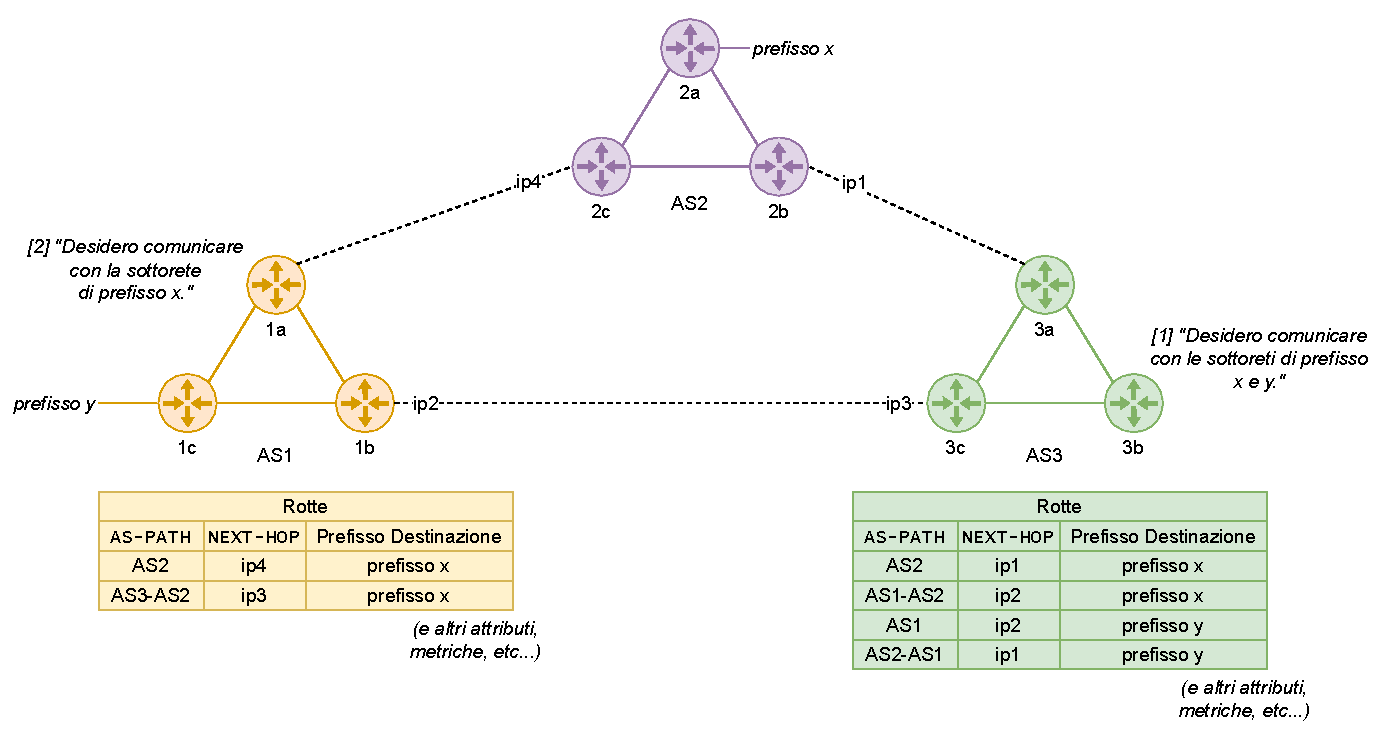
\includegraphics[width=1\linewidth]{./images/BGP.pdf}
\end{figure}

Supponiamo si voglia \textbf{dichiarare la raggiungibilità del prefisso $x$}. L'annuncio di raggiungibilità verrà passato ai nodi adiacenti, che costruiranno una tabella BGP contenente alcuni attributi, tra cui:
\begin{itemize}
	\item \verb|AS-PATH|: indica i sistemi autonomi tramite cui è passato questo annuncio.
	\item \verb|NEXT-HOP|: indica l'IP dell'interfaccia di rete tramite cui "entrare" nel primo sistema autonomo dell'\verb|AS-PATH|.
	\item Il prefisso $x$ da raggiungere.
\end{itemize}

L'insieme prefisso $x$ + attributi è detto \textit{route}, \textbf{rotta}. Valutando ogni \verb|NEXT-HOP| secondo una metrica stabilita, i router possono stabilire il percorso migliore.

\begin{footnotesize}
	\begin{verbatim}
		+------------+------------------------------------------+
		| Code Point |         Metric Type                      |
		+------------+------------------------------------------+
		|     0      | IGP Metric                               |
		|     1      | Min Unidirectional Link Delay [RFC7471]  |
		|     2      | TE Metric [RFC3630]                      |
		|     3      | Hop Count (refer [RFC5440])              |
		|     4      | SID List Length                          |
		|     5      | Loss Rate                                |
		|    6-250   | Unassigned                               |
		|  251-255   | Private Use (not to be assigned by IANA) |
		+------------+------------------------------------------+
		
		Figure 3: Metric Type Code Point  
	\end{verbatim}
\end{footnotesize}
